% =====================================================================
%  editor-formalism.tex
%
%  A formal account of an "ideal" (universal) WYSIWYG editor over the UI
%  tree  T = (N, r, p, chi, ell),  ell(n) = (tau, A, S, E, rho),  and of a
%  restricted sub-editor in which a fixed set of elements may be styled,
%  moved, and otherwise manipulated, but never removed.
%
%  Self-contained.  Compile with:   pdflatex editor-formalism.tex
%  (run twice so cross-references resolve).
%
%  Reuses the notation of tree-bracket.tex.  To open with that bracket
%  figure, put  % =====================================================================
%  Full-page nested-bracket hierarchy of a UI tree.
%
%  Containment encodes parent/descendant: a left bracket [ encloses a
%  node together with its whole subtree.  Each node sits at the TOP of
%  its own bracket; the bracket's bottom extends a fixed margin BELOW
%  its last child's bracket, so children nest neatly within the parent.
%  Depth = horizontal indent; preorder = vertical order.
%
%  Requires only \usepackage{tikz} and amssymb (\mathbb, \vartriangleleft).
% =====================================================================
% vertical bar + bottom serif of an elongated "["  (top = serif-to-label line)
\providecommand{\lbr}[4]{\draw[#1] (#2,#3) -- (#2,#4) -- ([xshift=4mm]#2,#4);}

\clearpage
\thispagestyle{empty}
\null\vfill
\noindent
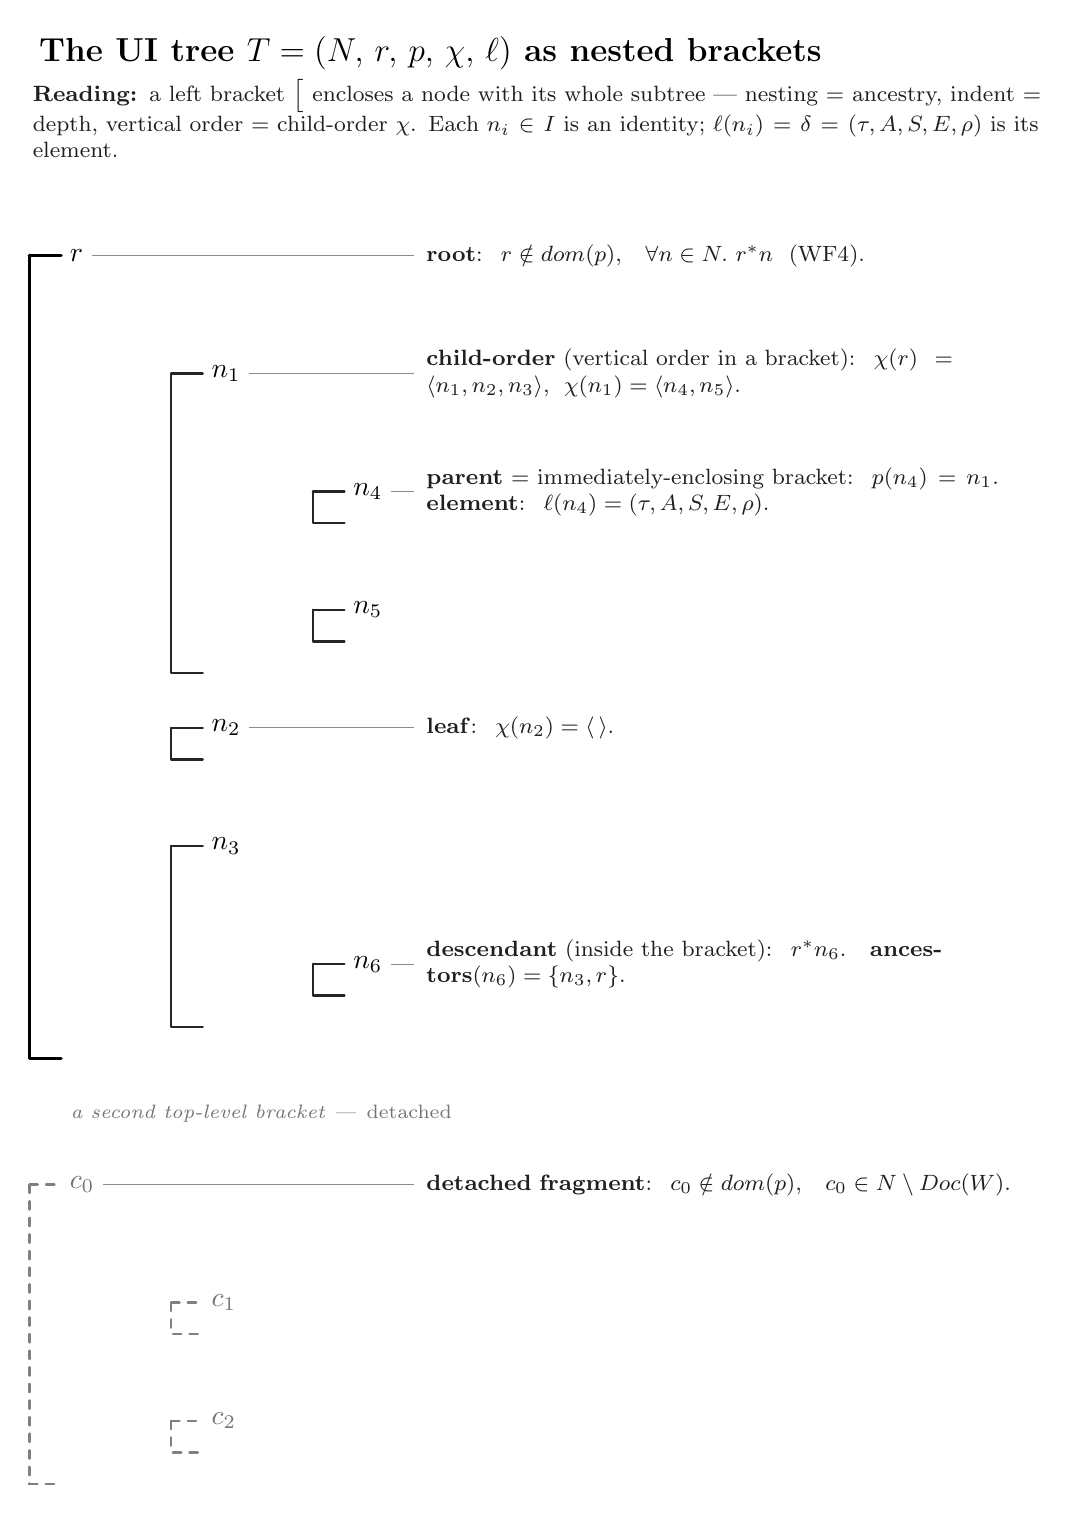
\begin{tikzpicture}[
  font=\footnotesize,
  nd/.style={anchor=west, inner xsep=3pt, inner ysep=1pt, font=\normalsize},
  ndd/.style={anchor=west, inner xsep=3pt, inner ysep=1pt, font=\normalsize, text=black!55},
  ann/.style={anchor=west, text width=7.6cm, align=left, font=\footnotesize,
              text=black!88, inner sep=1pt},
  leader/.style={draw=black!45, line width=.4pt},
  bk/.style={draw=black!85, line width=.9pt, line cap=round, line join=round},
  bkroot/.style={draw=black, line width=1.3pt, line cap=round, line join=round},
  bkd/.style={draw=black!50, line width=.9pt, dashed, line cap=round},
]

% ---------------- title + short reading guide ----------------
\node[font=\large\bfseries, anchor=north west] at (0,2.9)
  {The UI tree $T=(N,\,r,\,p,\,\chi,\,\ell)$ as nested brackets};
\node[ann, anchor=north west, text width=13.0cm] at (0,2.3)
  {\textbf{Reading:} a left bracket $\big[$ encloses a node with its whole subtree —
   nesting $=$ ancestry, indent $=$ depth, vertical order $=$ child-order $\chi$.
   Each $n_i\in\mathbb{I}$ is an identity; $\ell(n_i)=\delta=(\tau,A,S,E,\rho)$ is its element.};

% ---------------- node labels (sit on the top serif of each bracket) ----------------
\node[nd]  (r)  at (0.4,  0.0) {$r$};
\node[nd]  (n1) at (2.2, -1.5) {$n_1$};
\node[nd]  (n4) at (4.0, -3.0) {$n_4$};
\node[nd]  (n5) at (4.0, -4.5) {$n_5$};
\node[nd]  (n2) at (2.2, -6.0) {$n_2$};
\node[nd]  (n3) at (2.2, -7.5) {$n_3$};
\node[nd]  (n6) at (4.0, -9.0) {$n_6$};
\node[ndd] (c0) at (0.4,-11.8) {$c_0$};
\node[ndd] (c1) at (2.2,-13.3) {$c_1$};
\node[ndd] (c2) at (2.2,-14.8) {$c_2$};
\node[anchor=west, font=\scriptsize\itshape, text=black!55] at (0.4,-10.9)
  {a second top-level bracket — \emph{detached}};

% ---------------- brackets (bottom extends 0.4 below the last child's bottom) ----------------
\lbr{bkroot}{0}{0}{-10.2}       % r  : last child n3 closes at -9.8 -> r closes at -10.2
\lbr{bk}{1.8}{-1.5}{-5.3}       % n1 : last child n5 closes at -4.9 -> n1 closes at -5.3
\lbr{bk}{3.6}{-3.0}{-3.4}       % n4 (leaf)
\lbr{bk}{3.6}{-4.5}{-4.9}       % n5 (leaf, last child of n1)
\lbr{bk}{1.8}{-6.0}{-6.4}       % n2 (leaf)
\lbr{bk}{1.8}{-7.5}{-9.8}       % n3 : last child n6 closes at -9.4 -> n3 closes at -9.8
\lbr{bk}{3.6}{-9.0}{-9.4}       % n6 (leaf, last child of n3)
\lbr{bkd}{0}{-11.8}{-15.6}      % c0 : last child c2 closes at -15.2 -> c0 closes at -15.6
\lbr{bkd}{1.8}{-13.3}{-13.7}    % c1 (leaf)
\lbr{bkd}{1.8}{-14.8}{-15.2}    % c2 (leaf)

% ---------------- top serif: bracket corner --> label ----------------
\draw[bkroot] (0,0)    -- (r.west);
\draw[bk] (1.8,-1.5)   -- (n1.west);
\draw[bk] (3.6,-3.0)   -- (n4.west);
\draw[bk] (3.6,-4.5)   -- (n5.west);
\draw[bk] (1.8,-6.0)   -- (n2.west);
\draw[bk] (1.8,-7.5)   -- (n3.west);
\draw[bk] (3.6,-9.0)   -- (n6.west);
\draw[bkd] (0,-11.8)   -- (c0.west);
\draw[bkd] (1.8,-13.3) -- (c1.west);
\draw[bkd] (1.8,-14.8) -- (c2.west);

% ---------------- terse labels + relationships (leader stops ~1.2mm short) ----------------
\node[ann] (aRoot) at (5.0, 0.0)
  {\textbf{root}:\; $r\notin\operatorname{dom}(p)$,\quad $\forall n\in N.\ r\vartriangleleft^{*}n$ \ \textup{(WF4)}.};
\node[ann] (aChi) at (5.0,-1.5)
  {\textbf{child-order} (vertical order in a bracket):\; $\chi(r)=\langle n_1,n_2,n_3\rangle$,\; $\chi(n_1)=\langle n_4,n_5\rangle$.};
\node[ann] (aN4) at (5.0,-3.0)
  {\textbf{parent} $=$ immediately-enclosing bracket:\; $p(n_4)=n_1$.\quad \textbf{element}:\; $\ell(n_4)=(\tau,A,S,E,\rho)$.};
\node[ann] (aLeaf) at (5.0,-6.0)
  {\textbf{leaf}:\; $\chi(n_2)=\langle\,\rangle$.};
\node[ann] (aDesc) at (5.0,-9.0)
  {\textbf{descendant} (inside the bracket):\; $r\vartriangleleft^{*}n_6$.\quad \textbf{ancestors}$(n_6)=\{n_3,r\}$.};
\node[ann] (aFrag) at (5.0,-11.8)
  {\textbf{detached fragment}:\; $c_0\notin\operatorname{dom}(p)$,\quad $c_0\in N\setminus\operatorname{Doc}(W)$.};

\draw[leader] (r.east)  -- ([xshift=-1.2mm]aRoot.west);
\draw[leader] (n1.east) -- ([xshift=-1.2mm]aChi.west);
\draw[leader] (n4.east) -- ([xshift=-1.2mm]aN4.west);
\draw[leader] (n2.east) -- ([xshift=-1.2mm]aLeaf.west);
\draw[leader] (n6.east) -- ([xshift=-1.2mm]aDesc.west);
\draw[leader] (c0.east) -- ([xshift=-1.2mm]aFrag.west);

\end{tikzpicture}
\vfill
  where indicated in Section 1.
% =====================================================================
\documentclass[11pt]{article}

\usepackage[margin=1in]{geometry}
\usepackage{amsmath,amssymb,amsthm}
\usepackage{mathtools}
\usepackage{booktabs}
\usepackage{enumitem}
\usepackage{tikz}
\usetikzlibrary{positioning,arrows.meta}
\emergencystretch=1em   % absorb the odd minor overfull line

% ---- operators / notation matching tree-bracket.tex ----
\DeclareMathOperator{\Dom}{dom}
\DeclareMathOperator{\Doc}{Doc}
\DeclareMathOperator{\anc}{anc}
\newcommand{\II}{\mathbb{I}}                 % space of identities
\newcommand{\Tree}{\mathcal{T}}              % well-formed workspaces
\newcommand{\View}{\mathcal{V}}
\newcommand{\Edit}{\mathcal{E}}
\newcommand{\Ops}{\mathcal{O}}
\newcommand{\dle}{\vartriangleleft}          % immediate parent-of
\newcommand{\dleq}{\vartriangleleft^{*}}     % descendant (refl.-trans.)
\newcommand{\dlplus}{\vartriangleleft^{+}}   % proper descendant
\newcommand{\pfun}{\rightharpoonup}          % partial function
\newcommand{\coloniff}{\mathrel{:\Longleftrightarrow}}
\newcommand{\mint}{\mathsf{mint}}
\newcommand{\attach}{\mathsf{attach}}
\newcommand{\detach}{\mathsf{detach}}
\newcommand{\delete}{\mathsf{delete}}
\newcommand{\relabel}{\mathsf{relabel}}
\newcommand{\move}{\mathsf{move}}
\newcommand{\setType}{\mathsf{setType}}
\newcommand{\setStyle}{\mathsf{setStyle}}
\newcommand{\setAttr}{\mathsf{setAttr}}
\newcommand{\Wempty}{W_{\varnothing}}
\newcommand{\Render}{R}
\newcommand{\Lift}{L}
\newcommand{\step}[1]{\xrightarrow{\,#1\,}}
\newcommand{\stepP}[1]{\xrightarrow[P]{\,#1\,}}

% ---- theorem environments (shared counter) ----
\theoremstyle{definition}
\newtheorem{definition}{Definition}[section]
\newtheorem{remark}[definition]{Remark}
\theoremstyle{plain}
\newtheorem{theorem}[definition]{Theorem}
\newtheorem{proposition}[definition]{Proposition}

\title{An ideal WYSIWYG editor over a UI tree,\\[2pt]
       and its non-removable restriction}
\author{}
\date{}

\begin{document}
\maketitle

\begin{abstract}
We model an editor over the UI tree $T=(N,r,p,\chi,\ell)$ as a labelled
transition system on \emph{workspaces}. The ``ideal'' editor---one in which
\emph{anything} well-formed can be built---and a ``restricted'' editor---in which
a fixed handful of elements may be styled, moved, and otherwise manipulated but
never removed---are not different mechanisms. They are the same construction at
two ends of a lattice of invariants: the ideal editor is the top element,
constrained only by well-formedness, and a restricted editor is the
sub-transition-system carved out by a stronger invariant.
\end{abstract}

% =====================================================================
\section{The state space}
% =====================================================================
A \emph{workspace} is a tuple $W=(N,p,\chi,\ell,r)$ in which $(N,p)$ is a finite
forest, $r\in N$ a distinguished root, $\chi$ orders children, and $\ell$ labels
nodes by elements $\delta=(\tau,A,S,E,\rho)$. The \emph{document} is the part
reachable from $r$,
\[
  \Doc(W)\;\coloneqq\;\{\,n\in N : r\dleq n\,\},
\]
and the remaining forest-roots head \emph{detached fragments}, living in
$N\setminus\Doc(W)$ (the $c_0,c_1,c_2$ of the bracket figure). We write $\Tree$
for the set of \emph{well-formed} workspaces, those satisfying:

% To open with the nested-bracket picture, uncomment the next line:
% % =====================================================================
%  Full-page nested-bracket hierarchy of a UI tree.
%
%  Containment encodes parent/descendant: a left bracket [ encloses a
%  node together with its whole subtree.  Each node sits at the TOP of
%  its own bracket; the bracket's bottom extends a fixed margin BELOW
%  its last child's bracket, so children nest neatly within the parent.
%  Depth = horizontal indent; preorder = vertical order.
%
%  Requires only \usepackage{tikz} and amssymb (\mathbb, \vartriangleleft).
% =====================================================================
% vertical bar + bottom serif of an elongated "["  (top = serif-to-label line)
\providecommand{\lbr}[4]{\draw[#1] (#2,#3) -- (#2,#4) -- ([xshift=4mm]#2,#4);}

\clearpage
\thispagestyle{empty}
\null\vfill
\noindent
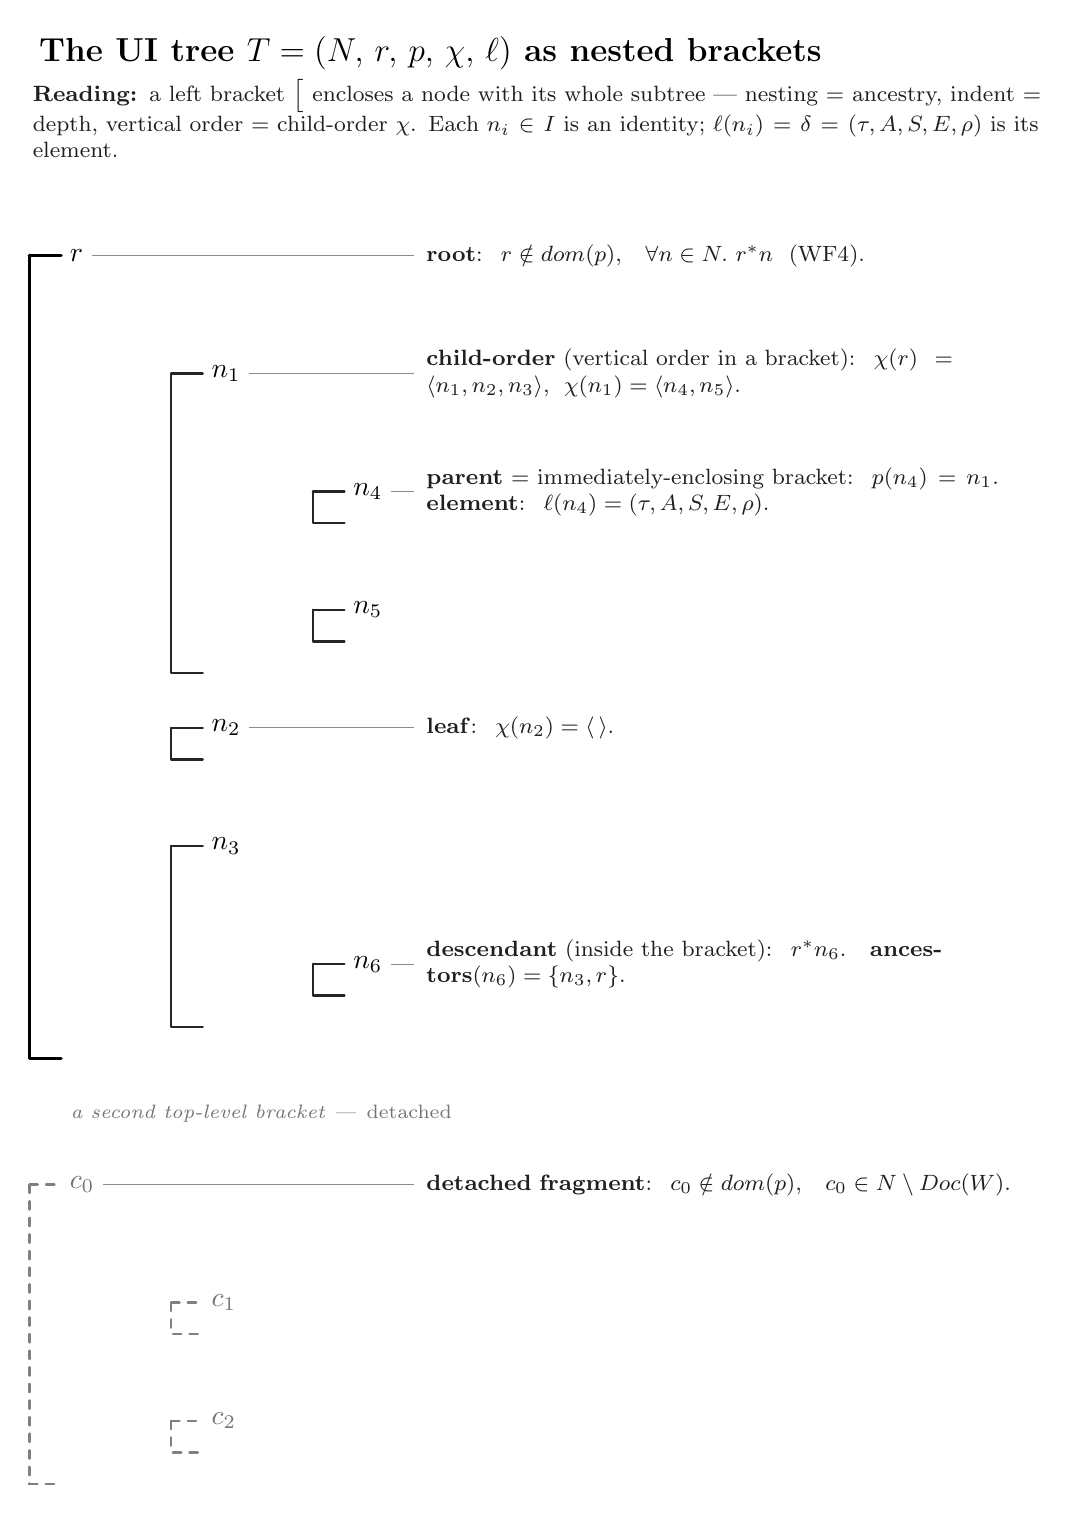
\begin{tikzpicture}[
  font=\footnotesize,
  nd/.style={anchor=west, inner xsep=3pt, inner ysep=1pt, font=\normalsize},
  ndd/.style={anchor=west, inner xsep=3pt, inner ysep=1pt, font=\normalsize, text=black!55},
  ann/.style={anchor=west, text width=7.6cm, align=left, font=\footnotesize,
              text=black!88, inner sep=1pt},
  leader/.style={draw=black!45, line width=.4pt},
  bk/.style={draw=black!85, line width=.9pt, line cap=round, line join=round},
  bkroot/.style={draw=black, line width=1.3pt, line cap=round, line join=round},
  bkd/.style={draw=black!50, line width=.9pt, dashed, line cap=round},
]

% ---------------- title + short reading guide ----------------
\node[font=\large\bfseries, anchor=north west] at (0,2.9)
  {The UI tree $T=(N,\,r,\,p,\,\chi,\,\ell)$ as nested brackets};
\node[ann, anchor=north west, text width=13.0cm] at (0,2.3)
  {\textbf{Reading:} a left bracket $\big[$ encloses a node with its whole subtree —
   nesting $=$ ancestry, indent $=$ depth, vertical order $=$ child-order $\chi$.
   Each $n_i\in\mathbb{I}$ is an identity; $\ell(n_i)=\delta=(\tau,A,S,E,\rho)$ is its element.};

% ---------------- node labels (sit on the top serif of each bracket) ----------------
\node[nd]  (r)  at (0.4,  0.0) {$r$};
\node[nd]  (n1) at (2.2, -1.5) {$n_1$};
\node[nd]  (n4) at (4.0, -3.0) {$n_4$};
\node[nd]  (n5) at (4.0, -4.5) {$n_5$};
\node[nd]  (n2) at (2.2, -6.0) {$n_2$};
\node[nd]  (n3) at (2.2, -7.5) {$n_3$};
\node[nd]  (n6) at (4.0, -9.0) {$n_6$};
\node[ndd] (c0) at (0.4,-11.8) {$c_0$};
\node[ndd] (c1) at (2.2,-13.3) {$c_1$};
\node[ndd] (c2) at (2.2,-14.8) {$c_2$};
\node[anchor=west, font=\scriptsize\itshape, text=black!55] at (0.4,-10.9)
  {a second top-level bracket — \emph{detached}};

% ---------------- brackets (bottom extends 0.4 below the last child's bottom) ----------------
\lbr{bkroot}{0}{0}{-10.2}       % r  : last child n3 closes at -9.8 -> r closes at -10.2
\lbr{bk}{1.8}{-1.5}{-5.3}       % n1 : last child n5 closes at -4.9 -> n1 closes at -5.3
\lbr{bk}{3.6}{-3.0}{-3.4}       % n4 (leaf)
\lbr{bk}{3.6}{-4.5}{-4.9}       % n5 (leaf, last child of n1)
\lbr{bk}{1.8}{-6.0}{-6.4}       % n2 (leaf)
\lbr{bk}{1.8}{-7.5}{-9.8}       % n3 : last child n6 closes at -9.4 -> n3 closes at -9.8
\lbr{bk}{3.6}{-9.0}{-9.4}       % n6 (leaf, last child of n3)
\lbr{bkd}{0}{-11.8}{-15.6}      % c0 : last child c2 closes at -15.2 -> c0 closes at -15.6
\lbr{bkd}{1.8}{-13.3}{-13.7}    % c1 (leaf)
\lbr{bkd}{1.8}{-14.8}{-15.2}    % c2 (leaf)

% ---------------- top serif: bracket corner --> label ----------------
\draw[bkroot] (0,0)    -- (r.west);
\draw[bk] (1.8,-1.5)   -- (n1.west);
\draw[bk] (3.6,-3.0)   -- (n4.west);
\draw[bk] (3.6,-4.5)   -- (n5.west);
\draw[bk] (1.8,-6.0)   -- (n2.west);
\draw[bk] (1.8,-7.5)   -- (n3.west);
\draw[bk] (3.6,-9.0)   -- (n6.west);
\draw[bkd] (0,-11.8)   -- (c0.west);
\draw[bkd] (1.8,-13.3) -- (c1.west);
\draw[bkd] (1.8,-14.8) -- (c2.west);

% ---------------- terse labels + relationships (leader stops ~1.2mm short) ----------------
\node[ann] (aRoot) at (5.0, 0.0)
  {\textbf{root}:\; $r\notin\operatorname{dom}(p)$,\quad $\forall n\in N.\ r\vartriangleleft^{*}n$ \ \textup{(WF4)}.};
\node[ann] (aChi) at (5.0,-1.5)
  {\textbf{child-order} (vertical order in a bracket):\; $\chi(r)=\langle n_1,n_2,n_3\rangle$,\; $\chi(n_1)=\langle n_4,n_5\rangle$.};
\node[ann] (aN4) at (5.0,-3.0)
  {\textbf{parent} $=$ immediately-enclosing bracket:\; $p(n_4)=n_1$.\quad \textbf{element}:\; $\ell(n_4)=(\tau,A,S,E,\rho)$.};
\node[ann] (aLeaf) at (5.0,-6.0)
  {\textbf{leaf}:\; $\chi(n_2)=\langle\,\rangle$.};
\node[ann] (aDesc) at (5.0,-9.0)
  {\textbf{descendant} (inside the bracket):\; $r\vartriangleleft^{*}n_6$.\quad \textbf{ancestors}$(n_6)=\{n_3,r\}$.};
\node[ann] (aFrag) at (5.0,-11.8)
  {\textbf{detached fragment}:\; $c_0\notin\operatorname{dom}(p)$,\quad $c_0\in N\setminus\operatorname{Doc}(W)$.};

\draw[leader] (r.east)  -- ([xshift=-1.2mm]aRoot.west);
\draw[leader] (n1.east) -- ([xshift=-1.2mm]aChi.west);
\draw[leader] (n4.east) -- ([xshift=-1.2mm]aN4.west);
\draw[leader] (n2.east) -- ([xshift=-1.2mm]aLeaf.west);
\draw[leader] (n6.east) -- ([xshift=-1.2mm]aDesc.west);
\draw[leader] (c0.east) -- ([xshift=-1.2mm]aFrag.west);

\end{tikzpicture}
\vfill


\begin{enumerate}[label=\textbf{WF\arabic*.}, leftmargin=*, itemsep=2pt]
  \item $p:N\pfun N$ is a partial function: every node has at most one parent.
  \item $\chi(n)$ is a duplicate-free sequence enumerating exactly $p^{-1}(n)$;
        thus $\chi$ is $p$ together with a sibling order.
  \item $\dlplus$ is irreflexive: the tree is acyclic and following $p$
        terminates. With WF1 this makes $(N,p)$ a forest.
  \item $r\notin\Dom(p)$ and $\Doc(W)$ is the $r$-reachable set
        (the root-reachability condition of the bracket figure).
  \item $\ell$ is total, and each $\delta=(\tau,A,S,E,\rho)$ is well-typed over a
        fixed tag alphabet.
\end{enumerate}

\begin{remark}[Schema]\label{rem:schema}
One may impose a sixth, optional constraint: a \emph{schema} $\Sigma$, a content
model fixing which types $\tau$ may parent which. This is the hinge of what
follows. ``Anything can be created'' is precisely the statement that $\Sigma$ is
trivial; the ideal editor is not powerful, it merely imposes nothing past
WF1--WF5. Any genuine schema is already a restriction of the kind developed in
Section~\ref{sec:restricted}.
\end{remark}

% =====================================================================
\section{The ideal editor}\label{sec:ideal}
% =====================================================================
An \emph{editor} is a labelled transition system $\Edit=(\mathcal S,\Ops,\to)$
with $\mathcal S\subseteq\Tree$ and each operation a \emph{partial function on
workspaces, defined only when its result again lies in $\Tree$}. The following
five operations generate everything.

\begin{enumerate}[label=\textup{(\arabic*)}, leftmargin=*, itemsep=3pt]
  \item $\mint(\delta)\Rightarrow n$: choose a fresh $n\notin N$, set
        $\ell(n)=\delta$, and leave $n$ parentless---a singleton fragment.
        \emph{Always defined.}
  \item $\attach(n,q,k)$: pre.\ $n$ is a fragment root, $q\in N$ lies outside the
        subtree of $n$ (no cycle), and $0\le k\le|\chi(q)|$. Sets $p(n)=q$ and
        inserts $n$ at index $k$ of $\chi(q)$.
  \item $\detach(n)$: pre.\ $n\in\Dom(p)$ and $n\ne r$. Removes $n$ from
        $\chi(p(n))$ and unsets $p(n)$; the subtree of $n$ leaves with it.
        \emph{Orphan, not destroy.}
  \item $\delete(n)$: pre.\ $n$ is a fragment root and $n\ne r$. Removes $n$
        (with its subtree) from $N$. \emph{Garbage-collect.}
  \item $\relabel(n,\delta')$: sets $\ell(n)=\delta'$; refine into
        $\setType,\setAttr,\setStyle,\dots$ to touch a single component of
        $\delta$.
\end{enumerate}

Write $\move(n,q,k)\coloneqq\detach(n);\,\attach(n,q,k)$ for the derived
reparent/reorder (with $q=p(n)$ a pure reorder), and call the generating set
\[
  \Ops_{\top}\;=\;\{\mint,\attach,\detach,\delete,\relabel\}.
\]
The separation of $\detach$ (remove from view) from $\delete$ (destroy) is what
makes the restriction of Section~\ref{sec:restricted} clean.

\begin{theorem}[Universality]\label{thm:univ}
From the seed $\Wempty$ (a single root $r$), the set reachable under
$\Ops_{\top}$ is exactly $\Tree$, and the reachability graph is strongly
connected.
\end{theorem}

\begin{proof}[Proof sketch]
\emph{Soundness.} Each precondition forces the result back into WF1--WF5: $\mint$
adds an isolated labelled node; $\attach$, by its no-cycle precondition, keeps
the forest and updates $\chi$ consistently; $\detach$ splits off a subtree;
$\delete$ drops a whole tree; $\relabel$ touches only~$\ell$.

\emph{Completeness.} To realise a target $W^\star$, $\mint$ every node with its
target label, then visit the nodes in \emph{preorder} and $\attach$ each
non-root beneath its target parent---preorder guarantees the parent is already
present---inserting at the target index. Detached fragments are rebuilt the same
way.

\emph{Strong connectivity.} From any $W$, repeatedly $\detach$ a leaf and
$\delete$ it, reaching $\Wempty$; composing with the build sequence reaches any
$W'$.
\end{proof}

Thus ``an ideal WYSIWYG editor such that anything can be created'' unfolds into
\emph{soundness} (every operation preserves $\Tree$) together with
\emph{completeness} (reachable $=\Tree$), under the trivial schema of
Remark~\ref{rem:schema}.

% =====================================================================
\section{The non-removable restriction}\label{sec:restricted}
% =====================================================================
Fix a finite set of \emph{protected identities} $P\subseteq\II$---the small,
manipulable-but-permanent set---optionally with frozen types
$\theta\colon P\to\mathrm{Tag}$. The entire restriction is one invariant on the
\emph{successor} state.

\begin{definition}[Protected invariant and restricted steps]\label{def:phi}
\begin{align*}
  \Phi^{\theta}_{P}(W)\;&\coloniff\;
     P\subseteq\Doc(W)\;\wedge\;\forall p\in P.\;\tau(\ell(p))=\theta(p),\\[2pt]
  W\stepP{e}W'\;&\coloniff\;\bigl(W\step{e}W'\bigr)\;\wedge\;\Phi^{\theta}_{P}(W').
\end{align*}
\end{definition}

That single condition needs no separate per-operation blocklist; reading it off
each operation yields Table~\ref{tab:perm}.

\begin{table}[h]
\centering
\begin{tabular}{@{}lll@{}}
\toprule
operation & effect on a $P$-node & outcome \\
\midrule
$\delete$                       & drops it from $N\supseteq\Doc$       & \textbf{blocked} (cannot remove)\\
$\detach$                       & moves it out of $\Doc$               & \textbf{blocked} (cannot orphan)\\
$\detach$ of an \emph{ancestor} & carries a $P$-node out of $\Doc$     & \textbf{blocked}\\
$\move$ to an in-document parent& subtree stays in $\Doc$              & \textbf{allowed} (``moved'')\\
$\setStyle,\ \setAttr$          & membership and type untouched        & \textbf{allowed} (``styled'')\\
$\setType$ to $\tau'\ne\theta(p)$ & breaks the type clause             & \textbf{blocked} (role frozen)\\
any op on a non-$P$ node, $\mint$ & cannot threaten $\Phi$             & \textbf{allowed} (free)\\
\bottomrule
\end{tabular}
\caption{Permissions induced by $\Phi^{\theta}_{P}$.}
\label{tab:perm}
\end{table}

The third row is the non-obvious consequence worth naming.

\begin{proposition}[Removability propagates upward]\label{prop:anc}
Under $\stepP{\,}$ the nodes that can no longer be detached or deleted are
exactly the ancestor-closure of $P$,
\[
  \anc^{*}(P)\;=\;\{\,m\in N : \exists\,p\in P.\; m\dleq p\,\},
\]
since orphaning any such $m$ would carry a protected node out of the document.
Protecting a node therefore freezes the removability of its entire ancestor
chain, while leaving each protected node free to move downward or sideways
wherever WF permits.
\end{proposition}

\begin{theorem}[Restricted reachability]\label{thm:restr}
From any seed $W_0$ with $\Phi^{\theta}_{P}(W_0)$ (the protected identities are
\emph{given}, not minted), the set reachable under $\stepP{\,}$ is exactly
\[
  \{\,W\in\Tree : \Phi^{\theta}_{P}(W)\,\}.
\]
It is strongly connected within this invariant but can never leave it. Formally
this is the sub-transition-system induced by $\Phi^{\theta}_{P}$: keep only
states satisfying the invariant and only edges between them. That induced
subgraph is the precise meaning of ``a restricted subset of the ideal editor.''
\end{theorem}

\begin{proof}[Proof sketch]
The build/teardown argument of Theorem~\ref{thm:univ} goes through verbatim on
the non-protected part; protected nodes are never deleted, detached, or retyped,
and are repositioned only by $\move$, which preserves $\Phi^{\theta}_{P}$ by
Table~\ref{tab:perm}. Conversely any target satisfying the invariant is reached
by editing the non-protected structure and $\move$-ing the protected nodes into
place.
\end{proof}

For finer, per-element control, replace the global $P$ by a \emph{capability map}
\[
  \kappa\colon N \longrightarrow
  2^{\{\mathsf{remove},\,\mathsf{reparent},\,\mathsf{reorder},\,\mathsf{restyle},\,\mathsf{retype},\,\mathsf{addChild},\,\mathsf{rmChild}\}},
\]
permitting an operation of kind $\mathsf{k}$ on node $n$ iff
$\mathsf{k}\in\kappa(n)$. The protected set is the instance
$\kappa(p)=\{\mathsf{reparent},\mathsf{reorder},\mathsf{restyle}\}$ for $p\in P$
and $\kappa(n)=\mathsf{ALL}$ otherwise.

\begin{remark}[Carrying policy in the element]
The natural home for $\kappa$ is the element itself. If the fifth component
$\rho$ of $\delta=(\tau,A,S,E,\rho)$ carries (or is extended to carry) per-node
policy, the restricted editor is \emph{literally} the ideal editor reading
editability off each node's $\rho$, and ``locked'' status travels with the node
across moves.
\end{remark}

% =====================================================================
\section{The WYSIWYG qualifier}\label{sec:wysiwyg}
% =====================================================================
Equip the document with a \emph{render} $\Render\colon\Tree\to\View$ (layout and
paint of $\Doc(W)$, ignoring fragments). The user acts on the \emph{view} by
gestures $g$; a WYSIWYG editor supplies a \emph{lift} $\Lift$ sending $(W,g)$ to
an operation so that editing the rendered output \emph{is} editing the state:

\begin{center}
\begin{tikzpicture}[>=Stealth, node distance=30mm and 40mm]
  \node (W)  {$W$};
  \node (Wp) [right=of W] {$W'=W\cdot \Lift(W,g)$};
  \node (V)  [below=16mm of W]  {$\Render(W)$};
  \node (Vp) [below=16mm of Wp] {$\Render(W')$};
  \draw[->] (W)  -- node[above]{$\Lift(W,g)$} (Wp);
  \draw[->] (W)  -- node[left]{$\Render$} (V);
  \draw[->] (Wp) -- node[right]{$\Render$} (Vp);
  \draw[->] (V)  -- node[below]{$g$} (Vp);
\end{tikzpicture}
\end{center}
\[
  \Render\bigl(W\cdot \Lift(W,g)\bigr)\;=\;g\cdot \Render(W).
\]

``WYSIWYG \emph{and} anything-creatable'' then asks that $\Render$ be injective
on editing-relevant structure---no hidden state alters the picture without a
handle---and that $\Lift$ be total over the gestures needed to reach any view. At
that point the universality of Theorem~\ref{thm:univ} transports across
$\Render$ to give \emph{completeness of direct manipulation}: every renderable
view is reachable by gesture.

The restriction of Section~\ref{sec:restricted} surfaces honestly as
\emph{missing affordances}: for $p\in P$ the lift offers drag-to-restyle and
drag-to-reposition handles but no delete handle, because the lifted operation
would fail~$\Phi^{\theta}_{P}$.

\begin{remark}[Honest caveat]
True injectivity of $\Render$ is essentially always false---distinct states
render to identical pixels---so production WYSIWYG editors take $\Render$ against
a structured \emph{editing model} rather than the literal raster, and state the
square there.
\end{remark}

% =====================================================================
\section{Composing restrictions}\label{sec:compose}
% =====================================================================
Schema and protection are invariants of the same lattice and simply intersect:
the editor constrained by both is the sub-transition-system induced by
$\Phi^{\theta}_{P}\wedge\Sigma$. The ideal editor is the top, $\Phi\equiv\top$;
every editor one actually ships is some meet of invariants below it.

\begin{center}
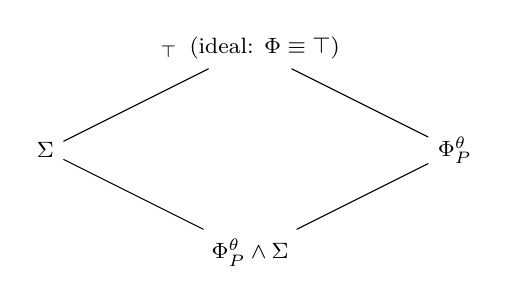
\begin{tikzpicture}[every node/.style={font=\footnotesize}, line cap=round]
  \node (top) at (0,2)      {$\Edit_{\top}$\, (ideal: $\Phi\equiv\top$)};
  \node (sig) at (-2.6,0.7) {$\Sigma$};
  \node (phi) at (2.6,0.7)  {$\Phi^{\theta}_{P}$};
  \node (bot) at (0,-0.6)   {$\Phi^{\theta}_{P}\wedge\Sigma$};
  \draw (top)--(sig); \draw (top)--(phi);
  \draw (sig)--(bot); \draw (phi)--(bot);
\end{tikzpicture}
\end{center}

\end{document}
